\documentclass[12pt]{article}
\usepackage[a4paper]{geometry}
\geometry{
    left = 20mm,
    right = 20mm,
    top = 20mm,
    bottom =20mm
}
\usepackage[skip=8pt, indent=20pt]{parskip}
\usepackage{fontspec}
\usepackage{dirtytalk}
\usepackage{hyphenat}
\usepackage{wrapfig}
\usepackage{booktabs}
\usepackage{float}
\usepackage{multicol}
\usepackage{caption}
\usepackage{subcaption}
\usepackage[shortlabels]{enumitem}
%\usepackage{natbib}
%\bibliographystyle{ksfh_nat}
\usepackage[toc,title,page]{appendix}
\usepackage{graphicx}
\graphicspath{ {./images/} }
\usepackage[export]{adjustbox}
\usepackage{hyperref}
\hypersetup{
    colorlinks=true,
    linkcolor=black,      
    urlcolor=blue
    }
\usepackage[dvipsnames]{xcolor}
\usepackage{amsmath}
\usepackage{amssymb}
\usepackage{mathrsfs}
\usepackage{mathdots}
\usepackage{dsfont}
\usepackage{upgreek}
\usepackage{tikz} % Podemos incluir librerías de de tikz \usetikzlibrari{positioning}
\usepackage{schemata}
\title{\vspace{-2cm}Strings and Gravity}
\author{José Manuel Begines Sánchez}
\date{9 de septiembre de 2023}
\linespread{1} % Interlineado

\setmainfont{Times New Roman}

\begin{document}
\maketitle
%\hrule
%\section*{\centering{Objectives}}
%\noindent This essay is aimed at concisely discussing String Theory as a theory of Quantum Gravity. I will talk about its historical motivations, its principles and assumptions, and its main results, most importantly how it incorporates a particle state which can be identified with the graviton.
%\vspace{0.55cm}
%\hrule

\section{Introduction}

Within the twentieth century, we can highlight two major breakthroughs in physics: Quantum Mechanics and General Relativity. General Relativity revolutionised the way we understood the space-time we live in, treating it as a dynamical entity, and allowed us to understand how our universe works at large scales. On the other hand, Quantum Mechanics have proved to be an essential tool to understand how physics works at microscopic scales, and indeed the evidence seems to indicate that nature follows the laws of quantum physics. However, while these two theoretical frameworks work astonishingly well on their own, an unification of both has proved to be a challenging task.

A straightforward attempt to combine quantum mechanics and general relativity is to interprete the latter as the low energy limit of an spin-2 massless quantum field within the framework of perturbative quantum field theory. And indeed, this is the case at least if we just consider the free theory. Once we try to incorporate interactions this theory turns out to be non-renormalizable.

To try to come up with a framework capable of describing the quantum aspects of gravity (while also being able to describe what we already know about the rest of interaction and matter fields), different areas have been developed, String Theory being the most promising one for the time being.

\section{String Theory}

Historically, particles have been understood as a point-like entity with characteristic properties (mass, charge, spin...). However, what string theory proposes is to think of particles as a one-dimensional object, "strings" that can be opened or closed (periodic boundary conditions). This strings, would have a characteristic tension \textquotedblleft$\mathcal{T}$\textquotedblright, which allow them to vibrate; and the properties of each particle would be encoded in their vibrational modes.

\begin{equation}\label{1}
    S = -\mathcal{T}\int_\Sigma dA
\end{equation}

Indeed, if we study the mechanics of a string with tension \textquotedblleft$\mathcal{T}$\textquotedblright, governed by the action of Equation (\ref{1}), where $\Sigma$ is the surface described by the string in its movement; and then quantize it, one is able to obtain a theory capable of describing particle physics. 

As a matter of fact, this theory started in the late 60s as an attempt to organize and give an explanation to the observed spectrum of hadrons and their interactions. However, this theory had some properties which prevented this particular application. The most relevant, considering that to its contemporary scope is not a problem, but a fundamental motivation; is that the theory imposes the existence of a massless spin-2 particle.

It wasn't until 1974 when Scherk and Schwarz suggested that we could interprete this mysterious massless spin-2 particle as the graviton, the quanta of the gravitational field, after proving that at low energies this "graviton", indeed interacted according to the covariance laws of general relativity \cite{Scherk:1974ca}. That is, General Relativity is a low energy limit of this quantum particle.

Not only does gravitons seams to exists within this framework, but they are unavoidable. To understand why this is the case, let's do an heuristic review of how String Theory works, from the point of view of path integrals. In the usual quantum field theory sense, one would have to derive the dynamics of a particle by summing over "all the possible paths" it could take, which would give us a probability amplitude. 

When particles are point-like this paths are known as world-lines, curves within space-time. However, when particles are thought as strings their movement does not describe a curve, but a surface, usually called "world-sheet". If we now consider interactions, we know that their description is governed by Feynman Diagrams in the usual quantum field theory, which we can understand as joining the paths of different particles. 

In the String Theory sense, interactions are thought similarly, as the joining and splitting of strings, which forms world-sheets with different topologies. However, while interactions in quantum-field theory need to be manually included, in string theory they are uniquely determined by the free theory. There are no arbitrary interactions to be chosen. 

Now, if we consider that our string interactions are local, then any theory of open strings necessarily contains closed strings \cite{Blumenhagen:2013fgp}, because two ends of strings will not know if they are part of the same string or not (non-localities within the theory would be mathematically inconsistent \cite{Polchinski:1998rq}).

\begin{figure}[h]
    \centering
    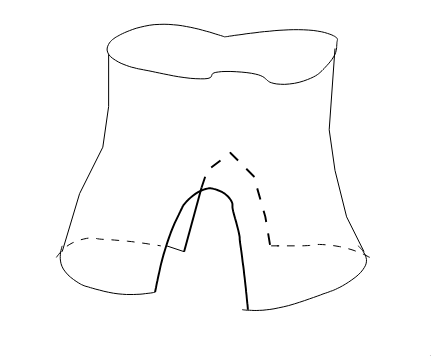
\includegraphics[width=0.4\textwidth]{uranga_closed_opened.png}
    \caption{World-sheet of two opened strings joining ends to become a closed one \cite{uranga}.}
\end{figure}

Gravitons within String Theory arise as a normal mode of a closed string. Then, the conclusion of the last paragraph imply that any string theory of particles we could construct requiere the existence of gravity; whereas ordinary quantum field theory "breaks" when we try to introduce gravity in it \cite{Becker:2006dvp}.

A way to heuristically explain why the unavoidable infinite probability amplitudes, that gravity produces in quantum field theory, are not present in string theory is the fact that interactions within this framework are not related to short-distance singularities, we do not have instantaneous emission and absorption of particles, this interactions are gradual. We could say that the string scale $1/l_s$ (where "$l_s$" is the characteristic size of strings), acts as a UV cutoff that prevents these divergences.

So far, this theory looks really promising: it explains why there are different types of particles, it predict that they can interact and most importantly, it includes a quantum description of gravity. However, everything I have discussed so far exhibits three main problems. 

First of all, every string within this theory behaves like bosons. The theory as I have briefly formulated is known as bossonic string theory. The second problem is that this theory predicts the unavoidable existence of "tachyons", particles which would have imaginary masses, a mathematical problem that would make our model unstable. The last problem is that this theory only works with a space-time of 26 dimensions. With all this problems, string theory seams to be quite far from describing our universe.

\section{Superstring Theory and its Predictions}

To try to solve the problems I outlined in the last paragraph of the previous sections, the theory must be pushed a bit further. To do so, we must consider strings which can have spin degrees of freedom. A way to think about this, is to consider that we are adding spinnors to the strings \cite{Ortin:2015hya}.

This indeed allow us to obtain particles which acts as fermions. What's more, this new theory gets rid of this "tachyons" which were unavoidable in the bosonic case. However, we still have some problems to face. Firstly, the critical dimension of this theory is 10; which, although lower than the 26 dimensions of bosonic string theory, is far more than our 4 space-time dimensions. Additionally, this theory predicts that there should exists the same number of fermions and bosons (Supersymmetry), a prediction that is far from observed considering our current Standard Model of Particles.

The first problem of dimensions is being mainly faced with the concept of compactification. This concept considers that the extra dimensions length scale would be \textquotedblleft small\textquotedblright compared to that of the usual 4 space-time dimensions, so that seen from afar they would not be noticed. Another proposition is that we could be living within a 4-dimesional brane of this higher-dimesional space-time that string theory predicts. This last proposition would roughly explain why gravity is so weak compared to the other fundamental forces: while the electromagnetic, weak and strong interactions would be localized on our brane, gravity would have to propagate through the whole of this 10 dimensional space-time.

On the other hand, supersymmetry not being detected could be accounted for experimental limitations. "We (may) need bigger colliders", as particle physicist would say. Further insight may be expected once the FCC (Future Circular Collider) starts to operate in the mid-2040s \cite{Suarez:2022pcn}. 

Lastly, I'd like to point out one test of String Theory closely related to gravity. Gravitons low energy limit does not only give us General Relativity, but it also predicts higher order terms which would "modify" gravity. Then, if we were to detect deviations from General Relativity predictions in astrophysical observation, we could see if String Theory can account for them. For example, the analysis of "Times-of-Arrival" of binary pulsars is being used to constraint this theories of this "Modified Gravity" \cite{Stairs:2005ai}.


\bibliographystyle{elsarticle-num}
\bibliography{reference.bib}

\end{document}
